\documentclass[border=10pt]{standalone}
\usepackage{pgfplots}
\pgfplotsset{compat=1.18}

\begin{document}
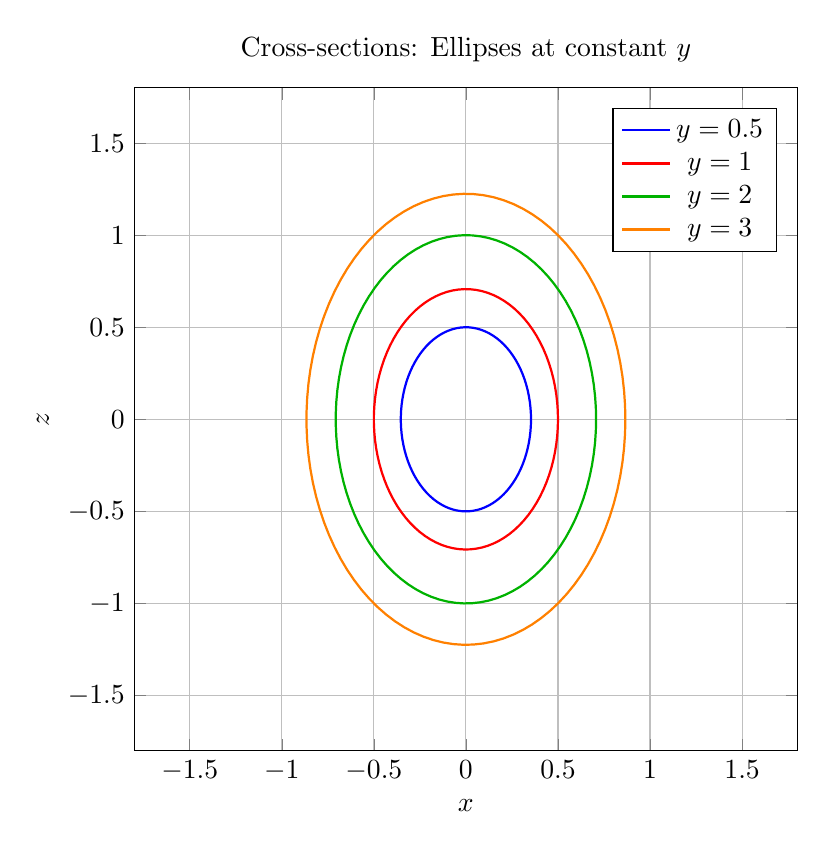
\begin{tikzpicture}
\begin{axis}[
    width=10cm,
    height=10cm,
    xlabel=$x$,
    ylabel=$z$,
    title={Cross-sections: Ellipses at constant $y$},
    axis equal,
    grid=major,
    xmin=-1.2,
    xmax=1.2,
    ymin=-1.8,
    ymax=1.8,
    legend pos=north east,
]
% y = 0.5
\addplot[domain=0:360, samples=100, blue, thick] ({sqrt(0.5/4)*cos(x)}, {sqrt(0.5/2)*sin(x)});
\addlegendentry{$y = 0.5$}

% y = 1
\addplot[domain=0:360, samples=100, red, thick] ({sqrt(1/4)*cos(x)}, {sqrt(1/2)*sin(x)});
\addlegendentry{$y = 1$}

% y = 2
\addplot[domain=0:360, samples=100, green!70!black, thick] ({sqrt(2/4)*cos(x)}, {sqrt(2/2)*sin(x)});
\addlegendentry{$y = 2$}

% y = 3
\addplot[domain=0:360, samples=100, orange, thick] ({sqrt(3/4)*cos(x)}, {sqrt(3/2)*sin(x)});
\addlegendentry{$y = 3$}
\end{axis}
\end{tikzpicture}
\end{document}